% Options for packages loaded elsewhere
\PassOptionsToPackage{unicode}{hyperref}
\PassOptionsToPackage{hyphens}{url}
\PassOptionsToPackage{dvipsnames,svgnames,x11names}{xcolor}
%
\documentclass[
  letterpaper,
  DIV=11,
  numbers=noendperiod]{scrartcl}

\usepackage{amsmath,amssymb}
\usepackage{iftex}
\ifPDFTeX
  \usepackage[T1]{fontenc}
  \usepackage[utf8]{inputenc}
  \usepackage{textcomp} % provide euro and other symbols
\else % if luatex or xetex
  \usepackage{unicode-math}
  \defaultfontfeatures{Scale=MatchLowercase}
  \defaultfontfeatures[\rmfamily]{Ligatures=TeX,Scale=1}
\fi
\usepackage{lmodern}
\ifPDFTeX\else  
    % xetex/luatex font selection
\fi
% Use upquote if available, for straight quotes in verbatim environments
\IfFileExists{upquote.sty}{\usepackage{upquote}}{}
\IfFileExists{microtype.sty}{% use microtype if available
  \usepackage[]{microtype}
  \UseMicrotypeSet[protrusion]{basicmath} % disable protrusion for tt fonts
}{}
\makeatletter
\@ifundefined{KOMAClassName}{% if non-KOMA class
  \IfFileExists{parskip.sty}{%
    \usepackage{parskip}
  }{% else
    \setlength{\parindent}{0pt}
    \setlength{\parskip}{6pt plus 2pt minus 1pt}}
}{% if KOMA class
  \KOMAoptions{parskip=half}}
\makeatother
\usepackage{xcolor}
\setlength{\emergencystretch}{3em} % prevent overfull lines
\setcounter{secnumdepth}{-\maxdimen} % remove section numbering
% Make \paragraph and \subparagraph free-standing
\ifx\paragraph\undefined\else
  \let\oldparagraph\paragraph
  \renewcommand{\paragraph}[1]{\oldparagraph{#1}\mbox{}}
\fi
\ifx\subparagraph\undefined\else
  \let\oldsubparagraph\subparagraph
  \renewcommand{\subparagraph}[1]{\oldsubparagraph{#1}\mbox{}}
\fi

\usepackage{color}
\usepackage{fancyvrb}
\newcommand{\VerbBar}{|}
\newcommand{\VERB}{\Verb[commandchars=\\\{\}]}
\DefineVerbatimEnvironment{Highlighting}{Verbatim}{commandchars=\\\{\}}
% Add ',fontsize=\small' for more characters per line
\usepackage{framed}
\definecolor{shadecolor}{RGB}{241,243,245}
\newenvironment{Shaded}{\begin{snugshade}}{\end{snugshade}}
\newcommand{\AlertTok}[1]{\textcolor[rgb]{0.68,0.00,0.00}{#1}}
\newcommand{\AnnotationTok}[1]{\textcolor[rgb]{0.37,0.37,0.37}{#1}}
\newcommand{\AttributeTok}[1]{\textcolor[rgb]{0.40,0.45,0.13}{#1}}
\newcommand{\BaseNTok}[1]{\textcolor[rgb]{0.68,0.00,0.00}{#1}}
\newcommand{\BuiltInTok}[1]{\textcolor[rgb]{0.00,0.23,0.31}{#1}}
\newcommand{\CharTok}[1]{\textcolor[rgb]{0.13,0.47,0.30}{#1}}
\newcommand{\CommentTok}[1]{\textcolor[rgb]{0.37,0.37,0.37}{#1}}
\newcommand{\CommentVarTok}[1]{\textcolor[rgb]{0.37,0.37,0.37}{\textit{#1}}}
\newcommand{\ConstantTok}[1]{\textcolor[rgb]{0.56,0.35,0.01}{#1}}
\newcommand{\ControlFlowTok}[1]{\textcolor[rgb]{0.00,0.23,0.31}{#1}}
\newcommand{\DataTypeTok}[1]{\textcolor[rgb]{0.68,0.00,0.00}{#1}}
\newcommand{\DecValTok}[1]{\textcolor[rgb]{0.68,0.00,0.00}{#1}}
\newcommand{\DocumentationTok}[1]{\textcolor[rgb]{0.37,0.37,0.37}{\textit{#1}}}
\newcommand{\ErrorTok}[1]{\textcolor[rgb]{0.68,0.00,0.00}{#1}}
\newcommand{\ExtensionTok}[1]{\textcolor[rgb]{0.00,0.23,0.31}{#1}}
\newcommand{\FloatTok}[1]{\textcolor[rgb]{0.68,0.00,0.00}{#1}}
\newcommand{\FunctionTok}[1]{\textcolor[rgb]{0.28,0.35,0.67}{#1}}
\newcommand{\ImportTok}[1]{\textcolor[rgb]{0.00,0.46,0.62}{#1}}
\newcommand{\InformationTok}[1]{\textcolor[rgb]{0.37,0.37,0.37}{#1}}
\newcommand{\KeywordTok}[1]{\textcolor[rgb]{0.00,0.23,0.31}{#1}}
\newcommand{\NormalTok}[1]{\textcolor[rgb]{0.00,0.23,0.31}{#1}}
\newcommand{\OperatorTok}[1]{\textcolor[rgb]{0.37,0.37,0.37}{#1}}
\newcommand{\OtherTok}[1]{\textcolor[rgb]{0.00,0.23,0.31}{#1}}
\newcommand{\PreprocessorTok}[1]{\textcolor[rgb]{0.68,0.00,0.00}{#1}}
\newcommand{\RegionMarkerTok}[1]{\textcolor[rgb]{0.00,0.23,0.31}{#1}}
\newcommand{\SpecialCharTok}[1]{\textcolor[rgb]{0.37,0.37,0.37}{#1}}
\newcommand{\SpecialStringTok}[1]{\textcolor[rgb]{0.13,0.47,0.30}{#1}}
\newcommand{\StringTok}[1]{\textcolor[rgb]{0.13,0.47,0.30}{#1}}
\newcommand{\VariableTok}[1]{\textcolor[rgb]{0.07,0.07,0.07}{#1}}
\newcommand{\VerbatimStringTok}[1]{\textcolor[rgb]{0.13,0.47,0.30}{#1}}
\newcommand{\WarningTok}[1]{\textcolor[rgb]{0.37,0.37,0.37}{\textit{#1}}}

\providecommand{\tightlist}{%
  \setlength{\itemsep}{0pt}\setlength{\parskip}{0pt}}\usepackage{longtable,booktabs,array}
\usepackage{calc} % for calculating minipage widths
% Correct order of tables after \paragraph or \subparagraph
\usepackage{etoolbox}
\makeatletter
\patchcmd\longtable{\par}{\if@noskipsec\mbox{}\fi\par}{}{}
\makeatother
% Allow footnotes in longtable head/foot
\IfFileExists{footnotehyper.sty}{\usepackage{footnotehyper}}{\usepackage{footnote}}
\makesavenoteenv{longtable}
\usepackage{graphicx}
\makeatletter
\def\maxwidth{\ifdim\Gin@nat@width>\linewidth\linewidth\else\Gin@nat@width\fi}
\def\maxheight{\ifdim\Gin@nat@height>\textheight\textheight\else\Gin@nat@height\fi}
\makeatother
% Scale images if necessary, so that they will not overflow the page
% margins by default, and it is still possible to overwrite the defaults
% using explicit options in \includegraphics[width, height, ...]{}
\setkeys{Gin}{width=\maxwidth,height=\maxheight,keepaspectratio}
% Set default figure placement to htbp
\makeatletter
\def\fps@figure{htbp}
\makeatother

\KOMAoption{captions}{tableheading}
\makeatletter
\makeatother
\makeatletter
\makeatother
\makeatletter
\@ifpackageloaded{caption}{}{\usepackage{caption}}
\AtBeginDocument{%
\ifdefined\contentsname
  \renewcommand*\contentsname{Table of contents}
\else
  \newcommand\contentsname{Table of contents}
\fi
\ifdefined\listfigurename
  \renewcommand*\listfigurename{List of Figures}
\else
  \newcommand\listfigurename{List of Figures}
\fi
\ifdefined\listtablename
  \renewcommand*\listtablename{List of Tables}
\else
  \newcommand\listtablename{List of Tables}
\fi
\ifdefined\figurename
  \renewcommand*\figurename{Figure}
\else
  \newcommand\figurename{Figure}
\fi
\ifdefined\tablename
  \renewcommand*\tablename{Table}
\else
  \newcommand\tablename{Table}
\fi
}
\@ifpackageloaded{float}{}{\usepackage{float}}
\floatstyle{ruled}
\@ifundefined{c@chapter}{\newfloat{codelisting}{h}{lop}}{\newfloat{codelisting}{h}{lop}[chapter]}
\floatname{codelisting}{Listing}
\newcommand*\listoflistings{\listof{codelisting}{List of Listings}}
\makeatother
\makeatletter
\@ifpackageloaded{caption}{}{\usepackage{caption}}
\@ifpackageloaded{subcaption}{}{\usepackage{subcaption}}
\makeatother
\makeatletter
\@ifpackageloaded{tcolorbox}{}{\usepackage[skins,breakable]{tcolorbox}}
\makeatother
\makeatletter
\@ifundefined{shadecolor}{\definecolor{shadecolor}{rgb}{.97, .97, .97}}
\makeatother
\makeatletter
\makeatother
\makeatletter
\makeatother
\ifLuaTeX
  \usepackage{selnolig}  % disable illegal ligatures
\fi
\IfFileExists{bookmark.sty}{\usepackage{bookmark}}{\usepackage{hyperref}}
\IfFileExists{xurl.sty}{\usepackage{xurl}}{} % add URL line breaks if available
\urlstyle{same} % disable monospaced font for URLs
\hypersetup{
  pdftitle={Injustice Attention Report},
  pdfauthor={Tom Beesley},
  colorlinks=true,
  linkcolor={blue},
  filecolor={Maroon},
  citecolor={Blue},
  urlcolor={Blue},
  pdfcreator={LaTeX via pandoc}}

\title{Injustice Attention Report}
\author{Tom Beesley}
\date{}

\begin{document}
\maketitle
\ifdefined\Shaded\renewenvironment{Shaded}{\begin{tcolorbox}[borderline west={3pt}{0pt}{shadecolor}, enhanced, interior hidden, sharp corners, frame hidden, breakable, boxrule=0pt]}{\end{tcolorbox}}\fi

\hypertarget{setup-and-loading-in-the-data}{%
\subsection{Setup and loading in the
data}\label{setup-and-loading-in-the-data}}

\begin{Shaded}
\begin{Highlighting}[]
\FunctionTok{library}\NormalTok{(tidyverse)}
\end{Highlighting}
\end{Shaded}

\begin{verbatim}
-- Attaching core tidyverse packages ------------------------ tidyverse 2.0.0 --
v dplyr     1.1.1     v readr     2.1.4
v forcats   1.0.0     v stringr   1.5.0
v ggplot2   3.4.1     v tibble    3.2.1
v lubridate 1.9.2     v tidyr     1.3.0
v purrr     1.0.1     
-- Conflicts ------------------------------------------ tidyverse_conflicts() --
x dplyr::filter() masks stats::filter()
x dplyr::lag()    masks stats::lag()
i Use the conflicted package (<http://conflicted.r-lib.org/>) to force all conflicts to become errors
\end{verbatim}

\begin{Shaded}
\begin{Highlighting}[]
\FunctionTok{library}\NormalTok{(eyetools)}

\FunctionTok{load}\NormalTok{(}\StringTok{"inj\_unsw\_data.RData"}\NormalTok{)}

\NormalTok{eg\_stim }\OtherTok{\textless{}{-}} 
\NormalTok{  eg\_stim }\SpecialCharTok{\%\textgreater{}\%}
  \FunctionTok{mutate}\NormalTok{(}\AttributeTok{pNum =} \FunctionTok{as.numeric}\NormalTok{(pNum))}
\end{Highlighting}
\end{Shaded}

\hypertarget{setting-up-aois}{%
\subsection{Setting up AOIs}\label{setting-up-aois}}

\begin{Shaded}
\begin{Highlighting}[]
\CommentTok{\# Set AOIs}
\NormalTok{AOI\_stims }\OtherTok{\textless{}{-}} \FunctionTok{data.frame}\NormalTok{(}\FunctionTok{matrix}\NormalTok{(}\AttributeTok{nrow =} \DecValTok{3}\NormalTok{, }\AttributeTok{ncol =} \DecValTok{4}\NormalTok{))}
\FunctionTok{colnames}\NormalTok{(AOI\_stims) }\OtherTok{\textless{}{-}} \FunctionTok{c}\NormalTok{(}\StringTok{"x"}\NormalTok{, }\StringTok{"y"}\NormalTok{, }\StringTok{"width\_radius"}\NormalTok{, }\StringTok{"height"}\NormalTok{)}

\NormalTok{AOI\_stims[}\DecValTok{1}\NormalTok{,] }\OtherTok{\textless{}{-}} \FunctionTok{c}\NormalTok{(}\DecValTok{450}\NormalTok{, }\DecValTok{540}\NormalTok{, }\DecValTok{600}\NormalTok{, }\DecValTok{600}\NormalTok{) }\CommentTok{\# X, Y, W, H {-} left}
\NormalTok{AOI\_stims[}\DecValTok{2}\NormalTok{,] }\OtherTok{\textless{}{-}} \FunctionTok{c}\NormalTok{(}\DecValTok{1460}\NormalTok{, }\DecValTok{540}\NormalTok{, }\DecValTok{600}\NormalTok{, }\DecValTok{600}\NormalTok{) }\CommentTok{\# X, Y, W, H {-} right}
\NormalTok{AOI\_stims[}\DecValTok{3}\NormalTok{,] }\OtherTok{\textless{}{-}} \FunctionTok{c}\NormalTok{(}\DecValTok{960}\NormalTok{, }\DecValTok{540}\NormalTok{, }\DecValTok{200}\NormalTok{, }\DecValTok{200}\NormalTok{) }\CommentTok{\# X, Y, W, H {-} fixation}

\NormalTok{AOI\_stims\_names }\OtherTok{\textless{}{-}} \FunctionTok{c}\NormalTok{(}\StringTok{"left"}\NormalTok{, }\StringTok{"right"}\NormalTok{, }\StringTok{"centre"}\NormalTok{)}
\end{Highlighting}
\end{Shaded}

\hypertarget{number-of-fixations}{%
\section{Number of fixations}\label{number-of-fixations}}

Here's what a typical trial looks like with 25 fixations (using
\texttt{eyetools::spatial\_plot()}):

\begin{Shaded}
\begin{Highlighting}[]
\NormalTok{data\_trial }\OtherTok{\textless{}{-}} 
\NormalTok{  eg\_stim }\SpecialCharTok{\%\textgreater{}\%} 
  \FunctionTok{filter}\NormalTok{(pNum }\SpecialCharTok{==} \DecValTok{001}\NormalTok{, }
\NormalTok{         trial }\SpecialCharTok{==} \DecValTok{3}\NormalTok{)}

\NormalTok{eyetools}\SpecialCharTok{::}\FunctionTok{spatial\_plot}\NormalTok{(}\AttributeTok{fix\_data =}\NormalTok{ data\_trial, }
                       \AttributeTok{AOIs =}\NormalTok{ AOI\_stims)}
\end{Highlighting}
\end{Shaded}

\begin{figure}[H]

{\centering 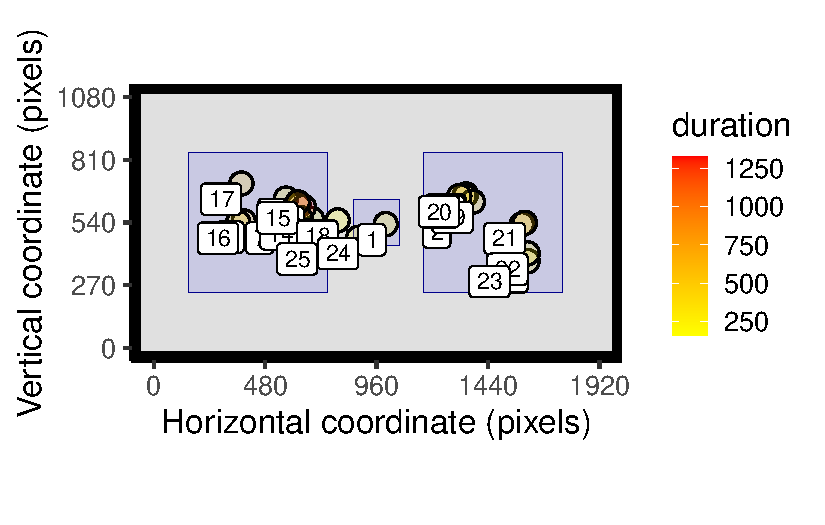
\includegraphics{inj_unsw_report_files/figure-pdf/unnamed-chunk-3-1.pdf}

}

\end{figure}

You can see from the index numbers that there is back and forth
processing between the two stimuli. We can use
\texttt{eyetools::AOI\_seq()} to look at how the eye movements entered
the different AOIs (here, just for the first 5 trials for this
participant):

\begin{Shaded}
\begin{Highlighting}[]
\NormalTok{data\_p1 }\OtherTok{\textless{}{-}} 
\NormalTok{  eg\_stim }\SpecialCharTok{\%\textgreater{}\%} 
  \FunctionTok{filter}\NormalTok{(pNum }\SpecialCharTok{==} \DecValTok{001}\NormalTok{)}

\NormalTok{eyetools}\SpecialCharTok{::}\FunctionTok{AOI\_seq}\NormalTok{(}\AttributeTok{data =}\NormalTok{ data\_p1, }\AttributeTok{AOIs =}\NormalTok{ AOI\_stims, }\AttributeTok{AOI\_names =}\NormalTok{ AOI\_stims\_names) }\SpecialCharTok{\%\textgreater{}\%} 
  \FunctionTok{head}\NormalTok{(}\DecValTok{5}\NormalTok{)}
\end{Highlighting}
\end{Shaded}

\begin{verbatim}
  trial                                     AOI_entry_seq
1     1 centre;right;centre;right;left;right;centre;right
2     2                centre;right;left;right;left;right
3     3    centre;right;left;right;left;right;centre;left
4     4                            centre;left;right;left
5     5          centre;left;right;left;centre;right;left
\end{verbatim}

Here's the distribution of number of fixations on a trial for all the
data:

\begin{Shaded}
\begin{Highlighting}[]
\NormalTok{eg\_stim }\SpecialCharTok{\%\textgreater{}\%} 
  \FunctionTok{group\_by}\NormalTok{(pNum, trial) }\SpecialCharTok{\%\textgreater{}\%} 
  \FunctionTok{summarise}\NormalTok{(}\AttributeTok{nFix =} \FunctionTok{n}\NormalTok{()) }\SpecialCharTok{\%\textgreater{}\%} 
  \FunctionTok{ggplot}\NormalTok{() }\SpecialCharTok{+}
  \FunctionTok{geom\_histogram}\NormalTok{(}\FunctionTok{aes}\NormalTok{(nFix), }\AttributeTok{bins =} \DecValTok{30}\NormalTok{, }\AttributeTok{fill =} \StringTok{"dark blue"}\NormalTok{) }\SpecialCharTok{+} 
  \FunctionTok{theme\_classic}\NormalTok{(}\AttributeTok{base\_size =} \DecValTok{12}\NormalTok{) }\SpecialCharTok{+}
  \FunctionTok{labs}\NormalTok{(}\AttributeTok{title =} \StringTok{"Distribution of number of fixations per trial"}\NormalTok{,}
       \AttributeTok{x =} \StringTok{"Number of fixations within a trial"}\NormalTok{,}
       \AttributeTok{y =} \StringTok{""}\NormalTok{)}
\end{Highlighting}
\end{Shaded}

\begin{verbatim}
`summarise()` has grouped output by 'pNum'. You can override using the
`.groups` argument.
\end{verbatim}

\begin{figure}[H]

{\centering 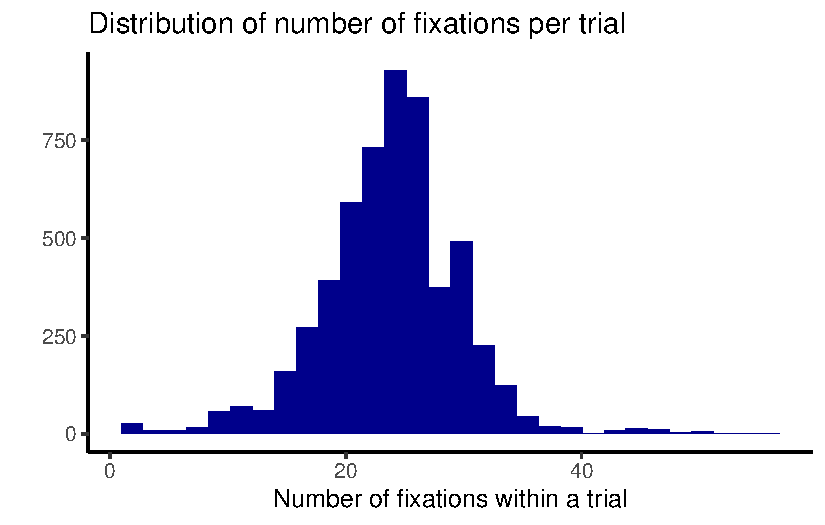
\includegraphics{inj_unsw_report_files/figure-pdf/unnamed-chunk-5-1.pdf}

}

\end{figure}

Do the participants vary much in the mean number of fixations per trial?



\end{document}
